\documentclass{article}
\usepackage{graphicx}
\usepackage{booktabs}
\usepackage{amsmath}
\usepackage{siunitx}
\usepackage{float}
\usepackage{pgfplots}

\usepackage{biblatex}
\addbibresource{resources.bib}

\usepackage{tikz}

\usepackage{pdfpages}

\DeclareSIUnit \irms {\ensuremath{\mathrm{A_{rms}}}}
\DeclareSIUnit \ipp {\ensuremath{\mathrm{A_{pp}}}}


\title{MPPT Inductor Design}
\author{Andrew Meares}
\date{2/7/2025}

\begin{document}

\maketitle

\section{Introduction}
In this paper we will design an inductor for an MPPT solar charge controller.
This inductor is for the buck converter topology MPPT tracker which is typical for high voltage arrays and lower voltage batteries.
We will first calculate the desired inductance, then we will select an appropriate core, analyze the copper losses and finally try to estimate the core losses.

\section{Calculate the Desired Inductance}

This inductor is for a buck converter that operates in continuous mode at high power.
The application is a versatile MPPT charge controller.
We will limit ourselves to foil wound powdered iron cores.

\subsection{Design Parameters}
The given input parameters are for a 200V maximum input voltage solar charge controller.  As an approximation of the maximum power operating point, we are going to use a lower input voltage of $\SI{152}{\volt}$.

\begin{align*}
    V_{\text{in}} &= \SI{152.0}{\volt} \\
    V_{\text{out}} &= \SI{54.0}{\volt} \\
    I_{\text{out}} &= \SI{50.0}{\ampere} \\
    f_{\text{sw}} &= \SI{30}{\kilo\hertz}
\end{align*}

\subsection{Duty Cycle}

The duty cycle \( D \) is given by Equation~\eqref{eq:duty}.

\begin{equation}
\label{eq:duty}
    D = \frac{V_{\text{out}}}{V_{\text{in}}} = \frac{\SI{54.0}{\volt}}{\SI{152.0}{\volt}} = \num{0.36}
\end{equation}

\subsection{Switching Time}

The on-time, \( T_{\text{on}} \), and off-time, \( T_{\text{off}} \), are calculated in Equations~\eqref{eq:ton} and \eqref{eq:toff}:

\begin{equation}
\label{eq:ton}
    T_{\text{on}} = \frac{D}{f_{\text{sw}}} = \frac{\num{0.36}}{\SI{30}{\kilo\hertz}} = \SI{12}{\micro\second}
\end{equation}

\begin{equation}
\label{eq:toff}
    T_{\text{off}} = \frac{1 - D}{f_{\text{sw}}} = \frac{1 - \num{0.36}}{\SI{30}{\kilo\hertz}} = \SI{21.3}{\micro\second}
\end{equation}

\subsection{Inductance Calculation}

The desired ripple factor is defined in Equation~\eqref{eq:rf}.

\begin{equation}
\label{eq:rf}
    RF = \frac{I_{\text{max}} - I_{\text{min}}}{I_{\text{avg}}} = \num{0.4}
\end{equation}

Equation~\eqref{eq:desl} gives the desired inductance value \cite[p. 26]{pressman2009}.

\begin{equation}
\label{eq:desl}
    L = \frac{(V_\text{in} - V_\text{out}) \cdot T_\text{on}}{I_\text{out} \cdot RF} = \SI{58.8}{\micro\henry}
\end{equation}

\section{Select an Appropriate Core}

To select an appropriate core, we consider the inductance factor \( A_L \) and the number of turns required to achieve the desired inductance.  To start, we will consider the Micro-Metals Kool Mu 00K5528E060 EE core set with \( A_L = \SI{219e-9}{\henry\per\tesla^2}\).

\subsection{Number of Turns Calculation}

The required number of whole turns \( N \) is determined by Equation~\eqref{eq:calcn}.

\begin{equation}
\label{eq:calcn}
    N = \sqrt{\frac{L}{A_L}} = \sqrt{\frac{\SI{58.0e-6}{\henry}}{\SI{219e-9}{\henry\per\tesla^2}}} = \num{16}
\end{equation}

\subsection{Inductance Verification}

The resulting calculated inductance \( L_\text{calc} \) is given by Equation~\eqref{eq:lcalc}.

\begin{equation}
\label{eq:lcalc}
    L_{\text{calc}} = A_L \times N^2 = (\SI{219e-9}{\henry\per\tesla^2}) \times \num{16}^2 = \SI{56.1}{\micro\henry}
\end{equation}

\subsection{DC Bias Calculation}

Equation~\eqref{eq:atcalc} calculates the ampere-turns (A-T) for the selected core at the given output current.

\begin{equation}
\label{eq:atcalc}
    A_T = I_{\text{out}} \times N = \SI{50}{\ampere} \times \num{17} = \SI{800}{\ampere\cdot\text{T}}
\end{equation}

This value is be compared to the core's DC bias performance curve shown in Figure \ref{fig:dcbias_5528} to ensure acceptable permeability under load. \\

\begin{figure}[H]
    \centering
    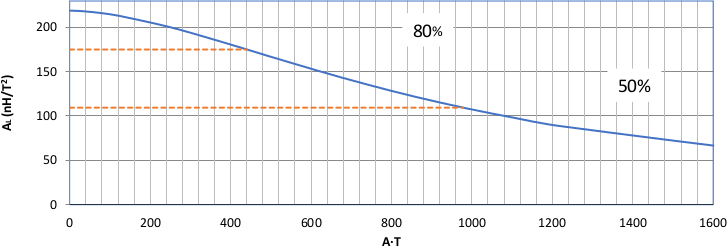
\includegraphics[height=4cm]{00K5528E060_dcbias_notitle.png}
    \caption{DC Bias Performance of Kool Mu $60\mu$ 5528 Core. Source: Manufacturer's datasheet.}
    \label{fig:dcbias_5528}
\end{figure}

I used engauge-digitizer and an image of the 00K5528E060 DC bias plot to craft a python interpolator that can return values along the DC bias plot curve.  For 16 turns, the \( A_L \) is significantly degraded.  It turns out 27 turns are required to get the desired inductance at the DC bias of 50A.  Here is my program output that iteratively calculates the required N.

\begin{verbatim}
L_desired: 0.000058
A_L at zero bias: 0.000000219440
Initial guess for N: 16
Iteration 1: N = 16, AT = 800.00, A_L = 0.000000128522, new_N = 21
Iteration 2: N = 21, AT = 1050.00, A_L = 0.000000103265, new_N = 24
Iteration 3: N = 24, AT = 1200.00, A_L = 0.000000090757, new_N = 25
Iteration 4: N = 25, AT = 1250.00, A_L = 0.000000086960, new_N = 26
Iteration 5: N = 26, AT = 1300.00, A_L = 0.000000083597, new_N = 26
Converged to N = 27

Calculated number of turns: 27
Calculated AT: 1350.0
Calculated A_L: 80.7
A_L 0 Bias: 219.4
Calculated A_L as % of A_L(0): 36.8%
Calculated inductance: 58.8 uH
\end{verbatim}

With this result, it is seen that this core size is too small for the desired value at a 50A DC bias current.  A more appropriate inductance value for 50A would be operating at 50\% saturation or less.  According to our chart, 50\% saturation occurs at 980 AT which is about 19 turns at 50A and would yield about 40 uH.

\begin{verbatim}
L_desired: 0.000040
A_L at zero bias: 0.000000219440
Initial guess for N: 14
Iteration 1: N = 14, AT = 700.00, A_L = 0.000000140926, new_N = 17
Iteration 2: N = 17, AT = 850.00, A_L = 0.000000123414, new_N = 18
Iteration 3: N = 18, AT = 900.00, A_L = 0.000000117907, new_N = 18
Converged to N = 19

Calculated number of turns: 19
Calculated AT: 950.0
Calculated A_L: 113.3
A_L 0 Bias: 219.4
Calculated A_L as % of A_L(0): 51.6%
Calculated inductance: 40.9 uH
\end{verbatim}

Working backwards, it can be determined that all other things held constant, 00K5528E060 would give us our ripple factor of 40\% with an appropriate DC bias at a minimum switching frequency.

\begin{equation}
    f_\text{min} = \frac{D \cdot (V_\text{in} - V_\text{out})}{\SI{40e-6}{\henry} \cdot I_\text{out} \cdot RF} = \SI{43520}{\hertz}
\end{equation}

\section{Kool Mu, 00K5530E060}

There is a core size that is slightly larger in volume, the 00K5530E060, with DC bias performance curve shown in Figure \ref{fig:dcbias_5530}.  Digitizing the DC bias performance curve and running the program yields the following output. \\

\begin{figure}[H]
    \centering
    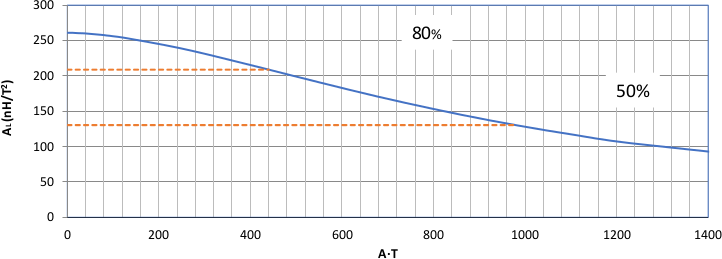
\includegraphics[height=4cm]{00K5530E060_dcbias_notitle.png}
    \caption{DC Bias Performance of Kool Mu $60\mu$ 5530 Core. Source: Manufacturer's datasheet.}
    \label{fig:dcbias_5530}
\end{figure}

\begin{verbatim}
L_desired: 0.000058
A_L at zero bias: 0.000000261900
Initial guess for N: 15
Iteration 1: N = 15, AT = 750.00, A_L = 0.000000161219, new_N = 19
Iteration 2: N = 19, AT = 950.00, A_L = 0.000000135155, new_N = 21
Iteration 3: N = 21, AT = 1050.00, A_L = 0.000000124424, new_N = 22
Iteration 4: N = 22, AT = 1100.00, A_L = 0.000000119060, new_N = 22
Iteration 5: N = 22, AT = 1100.00, A_L = 0.000000119060, new_N = 22

Calculated number of turns: 22
Calculated AT: 1100.0
Calculated A_L: 119.1
A_L 0 Bias: 261.9
Calculated A_L as % of A_L(0): 45.5%
Calculated inductance: 57.6 uH
\end{verbatim}

Again this core is a little small for 30kHz and 40\% RF.  Note that 30kHz is relatively fast for a low cost, high powered, Si FET half-bridge using 200V parts.  Also 40\% ripple factor is a lot of ripple.  This is telling me that our goal is ambitious.  We have not even considered yet how with 40\% peak to peak ripple, there is still 20\% more current at the peak of the switching cycle.  This will push the core further into saturation than recommended.

A maximum inductance for this core, still disregarding the "peak" current, is 47.3 uH.  Rerunning the switching frequency calculation yields a minimum frequency given by Equation~\eqref{eq:fmin1}.

\begin{equation}
\label{eq:fmin1}
    f_{\text{min}} = \frac{D \cdot (V_{\text{in}} - V_{\text{out}})}{\SI{40e-6}{\henry} \cdot I_{\text{out}} \cdot RF} = \SI{36803}{\hertz}
\end{equation}

\subsection{Kool Mu, 00K6527E060}
The next size up is 6527, which is nearly twice the volume as the 5528 size.
The 6527 core shows improved performance at high bias, as demonstrated in Figure \ref{fig:dcbias_6527}. \\

\begin{figure}[H]
    \centering
    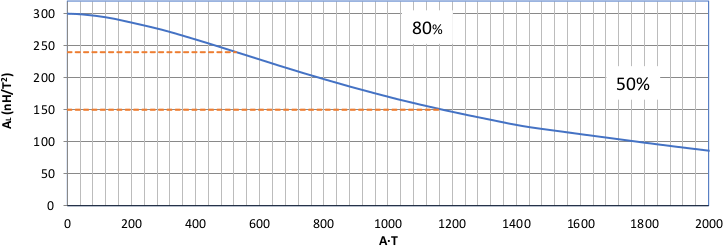
\includegraphics[height=4cm]{00K6527E060_dcbias_notitle.png}
    \caption{DC Bias Performance of Kool Mu $60\mu$ 6527 Core.  Source: Manufacturer's datasheet, included in Appendix~\ref{appendix:datasheets}.}
    \label{fig:dcbias_6527}
\end{figure}

\begin{verbatim}
L_desired: 0.000058
A_L at zero bias: 0.000000300680
Initial guess for N: 14
Iteration 1: N = 14, AT = 700.00, A_L = 0.000000212734, new_N = 17
Iteration 2: N = 17, AT = 850.00, A_L = 0.000000190965, new_N = 17
Converged to N = 18

Calculated number of turns: 18
Calculated AT: 900.0
Calculated A_L: 184.6
A_L 0 Bias: 300.7
Calculated A_L as % of A_L(0): 61.4%
Calculated inductance: 59.8 uH    
\end{verbatim}

The 00K6527E060 is looking like the right size.  This core operates at a 38.6\% saturation level at 50A.  This design is aggressive with no real margin to allow for higher peak currents.  This is somewhat on purpose because I have noticed that other MPPT designs tend to under-size the inductor, presumably to save cost.  Therefore, I am designing aggressively.

\subsection{Consider the Peak Current}

A more conservative design would be to allow for 20\% higher peak current and set the goal to not saturate more than say 50\% at that bias point.  Therefore instead of 50A DC bias, we will use 60A peak bias.

\begin{verbatim}
L_desired: 0.000058
A_L at zero bias: 0.000000300680
Initial guess for N: 14
Iteration 1: N = 14, AT = 840.00, A_L = 0.000000192216, new_N = 17
Iteration 2: N = 17, AT = 1020.00, A_L = 0.000000168122, new_N = 19
Iteration 3: N = 19, AT = 1140.00, A_L = 0.000000154153, new_N = 19
Converged to N = 20

Calculated number of turns: 20
Calculated AT: 1200.0
Calculated A_L: 146.6
A_L 0 Bias: 300.7
Calculated A_L as % of A_L(0): 48.8%
Calculated inductance: 58.6 uH
\end{verbatim}

This result indicates that adding 2 more turns will get us our inductance goal at the peak bias point as well.  Though I am not certain this is a better design choice.

Consider instead a design of 18 turns but the core saturates more than average during the peaks.  Here is an analysis of both bias points.

\begin{verbatim}
L_desired: 0.000058
A_L at zero bias: 0.000000300680
Initial guess for N: 14
Iteration 1: N = 14, AT = 700.00, A_L = 0.000000212734, new_N = 17
Iteration 2: N = 17, AT = 850.00, A_L = 0.000000190965, new_N = 17
Converged to N = 18

Calculated number of turns: 18
Calculated AT: 900.0
Calculated A_L: 184.6
Calculated A_L peak: 161.2
A_L 0 Bias: 300.7
Calculated A_L as % of A_L(0): 61.4%
Calculated A_L peak as % of A_L(0): 53.6%
Calculated inductance: 59.8 uH
Calculated min inductance at bias peak: 52.2 uH
\end{verbatim}

This indicates 18 turns is not a bad choice.  You get 38.6\% saturation on average and a peak saturation of less than 50\%.  The inductance is lower than the target at the peaks but not by a lot.

\subsection{Core Selection Results}
It turned out that a larger core, Mag-Inc 00K6527E060, is more appropriate for our inductor design.  The comparatively compact 00K5528E060 or 00K5530E060 cores require a higher switching frequency and lower target inductance to be a good fit.

Figure \ref{fig:inductance_vs_dc} shows the inductance and saturation level for each operating bias point.

\begin{figure}[H]
    \centering
    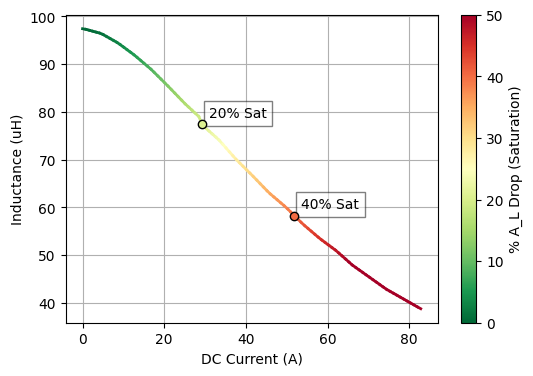
\includegraphics[height=6cm]{inductance_vs_dc_wsat_notitle.png}
    \caption{00K6527E060 inductance vs. $I_\text{bias}$ for 18 turns.}
    \label{fig:inductance_vs_dc}
\end{figure}

\section{Analyze the Copper}
These 18 turns around a 00K6527E060 EE core set will be made of copper foil.  There is a finite area that the foil can pass through to create a turn or winding.  This is called the window.  The window of the bare EE core set is reduced significantly by the bobbin which is made of sturdy plastic to prevent it from deforming under pressure from the winding.

In our case, we can use 00B652701, which is a standard bobbin for the 6527 core size.  From the bobbin drawing, we can ascertain that the width of the bobbin window is 39.5mm.  The bobbin window height is hard to ascertain from the drawing but the core window height is 12.09 mm and the plastic is on the order of 1mm thick with some extra slop for fit.  Lets say the bobbin window area is 39.5mm x 10.42mm.

Consider the 18 turns to make our inductor and our 50A average current.  We can calculate the current density of the window.  I will use the raw core window area.

\begin{equation}
    \text{Current Density} = \frac{\SI{50}{\ampere} \times \num{18}}{\SI{537}{\milli\meter\squared}} = \SI{1.7}{\ampere\per\milli\meter^2}
\end{equation}

We can also calculate how much area is available per turn.  This includes the insulation.

\begin{equation}
    A_\text{turn} = \frac{\SI{39.5}{\milli\meter\squared} \times \SI{10.42}{\milli\meter\squared}}{\num{18}} = \SI{22.9}{\milli\meter\squared}
\end{equation}

This copper cross sectional area is similar to 10 AWG wire.  Bending even 12 AWG round copper magnet wire is difficult, hence the choice of foil.

\subsection{Copper Foil}
Copper foil, annealed and edge-rolled, comes in multiple widths and thicknesses.
The foil must be insulated as it is wound around the bobbin.  Consider a generic insulation layer of a certain thickness for calculations.

The stackup of 10.42mm in height is part copper, part insulator, part air.  Consider an insulator+air that is 6mil or 0.152mm.  There are 18 layers of copper so 18 layers of insulator at least.  We will make the copper foil 0.2" or 5.08mm smaller in width than the bobbin. \\

\begin{figure}[H]
    \centering
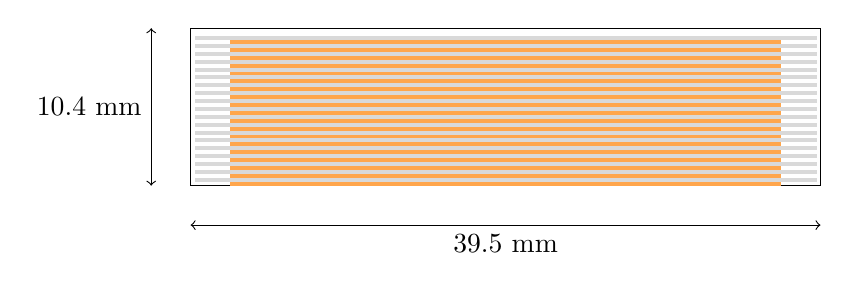
\begin{tikzpicture}

    % Define parameters
    \def\windowWidth{8}   % Scaled for better aspect ratio
    \def\windowHeight{2}
    \def\copperWidth{7}
    \def\insulatorWidth{7.9}
    \def\layerHeight{0.05}
    \def\nLayers{18} % Number of copper layers (ends with insulator on top)

    % Draw the window
    \draw[] (0,0) rectangle (\windowWidth, \windowHeight);

    % Draw the layers inside the window
    \foreach \i in {0,...,\nLayers} {
        \pgfmathsetmacro{\y}{\i * \layerHeight * 2}
        
        % Copper layer (bottom-most first)
        \fill[orange!70] 
            ({(\windowWidth - \copperWidth)/2}, \y) 
            rectangle 
            ({(\windowWidth + \copperWidth)/2}, \y + \layerHeight);
        
        % Insulator layer (slightly wider)
        \fill[gray!30] 
            ({(\windowWidth - \insulatorWidth)/2}, \y + \layerHeight) 
            rectangle 
            ({(\windowWidth + \insulatorWidth)/2}, \y + 2*\layerHeight);
    }

    % Dimension lines
    \draw[<->] (-0.5,0) -- (-0.5,\windowHeight) node[midway, left] {10.4 mm}; % Height dimension
    \draw[<->] (0,-0.5) -- (\windowWidth,-0.5) node[midway, below] {39.5 mm}; % Width dimension

\end{tikzpicture}
\caption{Cross-section of the inductor core window. Copper layers are represented in orange, while insulation is shown in gray.  Not to scale.}
    \label{fig:core_window}
\end{figure}

\begin{equation}
    H_{\text{ins}} = \num{18} \times \SI{0.152}{\milli\meter} = \SI{2.74}{\milli\meter}
\end{equation}

\begin{equation}
    H_{\text{bob}} \geq H_{\text{ins}} + H_{\text{Cu}}
\end{equation}

\begin{equation}
    H_{\text{foil}} \leq \frac{\SI{10.42}{\milli\meter} - \SI{2.74}{\milli\meter}}{\num{18}} = \SI{0.42}{\milli\meter} \text{ or } \SI{16.8}{\text{mil}}
\end{equation}

\begin{equation}
    A_{\text{foil}} = H_{\text{foil}} \times W_{\text{foil}} = \SI{0.42}{\milli\meter} \times (\SI{39.5}{\milli\meter} - \SI{5.08}{\milli\meter}) = \SI{14.5}{\milli\meter\squared} \text{ or } \SI{0.0225}{\text{in}^2}
\end{equation}

Our copper foil is equivalent to 12 AWG magnet wire in cross section.

\subsection{Fill Factor}
The fill factor is the percentage of the window that is filled with copper.  We are going to use the bare window size here.

\begin{equation}
FF = \frac{N \times A_\text{foil}}{A_\text{window}} = \frac{18 \times \SI{14.5}{\milli\meter\squared}}{\SI{537}{\milli\meter\squared}} = \SI{48.6}{\percent}
\end{equation}

A summary of how the window area is being utilized in our inductor is shown in Table \ref{tab:window_area}.

\begin{table}[H]
    \centering
    \begin{tabular}{l c}
        \hline
        Component & Window Area (\%) \\
        \hline
        Copper & \SI{48.6}{\percent} \\
        Air + Insulator & \SI{28.4}{\percent} \\
        Bobbin & \SI{23.0}{\percent} \\
        \hline
        Total & \SI{100.0}{\percent} \\
        \hline
    \end{tabular}
    \caption{Window area utilization in the inductor core.}
    \label{tab:window_area}
\end{table}

\subsection{Copper AC Losses}
We are going to ignore skin effect and proximity effect in this paper.  There is some justification for this.  Skin depth is 14.8mil at 30kHz, which is more than half the thickness of our copper foil, for one.  A second reason is that our ripple factor or AC component in our inductor current is "much" smaller than the DC component.  This is a bit of a stretch calling a 40\% ripple factor "much" smaller.  In a discontinuous mode design, pay more attention to these AC effects.

\subsection{How Long?}
Each turn makes the path around the rectangular bobbin longer.
Use the average of the short path and the longest path. \\

\begin{figure}[H]
    \centering
    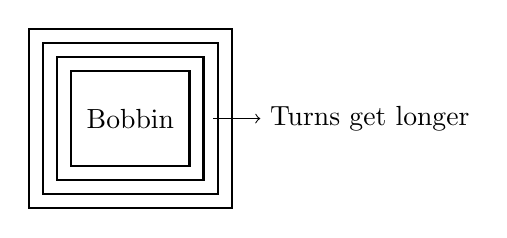
\begin{tikzpicture}[scale=0.6]

        % Define bobbin core dimensions (relative)
        \def\coreWidth{2.5}
        \def\coreHeight{2}
        \def\gap{0.3} % Gap between turns

        % Draw inner bobbin (first turn)
        \draw[thick] (-\coreWidth/2, -\coreHeight/2) 
                     rectangle (\coreWidth/2, \coreHeight/2)
                     node[pos=0.5] {Bobbin};

        % Draw a few layers (only 3 for clarity)
        \foreach \i in {1,2,3} {
            \pgfmathsetmacro{\w}{\coreWidth + 2*\i*\gap}
            \pgfmathsetmacro{\h}{\coreHeight + 2*\i*\gap}
            \draw[thick] (-\w/2, -\h/2) rectangle (\w/2, \h/2);
        }

        % Arrows showing turn length increase
        \draw[->] (\coreWidth/2 + 0.5, 0) -- (\coreWidth/2 + 1.5, 0) 
            node[right] {Turns get longer};

    \end{tikzpicture}
    \caption{Bobbin cross-section showing increasing turn length as winding layers build up.}
    \label{fig:bobbin_turns}
\end{figure}

\begin{equation}
    L_{\text{short}} = 2 \times \SI{30.3}{\milli\meter} + 2 \times \SI{23}{\milli\meter} = \SI{106.6}{\milli\meter}
\end{equation}

\begin{equation}
    L_{\text{long}} = 2 \times \SI{53}{\milli\meter} + 2 \times \SI{44.2}{\milli\meter} = \SI{194.4}{\milli\meter}
\end{equation}

\begin{equation}
    L_{\text{avg}} = \frac{1}{2} \left( \SI{106.6}{\milli\meter} + \SI{194.4}{\milli\meter} \right) = \SI{151}{\milli\meter}
\end{equation}

I discovered that in the back of the manufacturer's catalog, \cite[p. 197]{magincPowderCat2024}, the mean turn length is given for the 00B652701 bobbin as $\SI{168}{\milli\meter}$.  This value is 11\% larger than our estimate, so we will use the larger value. \\

When calculating the total length, add $\SI{100}{\milli\meter}$ for leads.

\begin{equation}
    L_{\text{total}} = \num{18} \times \SI{168}{\milli\meter} + \SI{100}{\milli\meter} = \SI{3124}{\milli\meter}
\end{equation}

\subsection{How Much Does it Weigh?}
The copper weight is given in Equation~\eqref{eq:cuweight}.  The density of copper is about $\SI{8.94}{\gram\per\centi\meter\cubed}$.
\begin{equation}
W_\text{Cu} = L_\text{total} H_\text{foil} W_\text{foil} D_\text{Cu}
\label{eq:cuweight}
\end{equation}
\begin{equation}
W_\text{Cu} = \SI{312.4}{\centi\meter} \times \SI{0.042}{\centi\meter} \times \SI{3.95}{\centi\meter} \times \SI{8.94}{\gram\per\centi\meter\cubed} = \SI{463}{\gram}
\end{equation}

\subsection{Copper Losses Estimate}
The resistivity of annealed copper is $\rho_{\text{Cu}} = 1.72 \times 10^{-8} \, \Omega\cdot\text{m}$.

\begin{equation}
    R = \rho \frac{L}{A} = \left(\SI{1.72e-8}{\ohm\meter} \right) \times \frac{\SI{3.124}{\meter}}{\SI{14.5e-6}{\meter\squared}} = \SI{0.0037}{\ohm}
\end{equation}

What are the losses for a 50A current?  Use the average for a quick estimate.

\begin{equation}
P_\text{Cu, iavg} = (50 \text{A})^2 \times 0.0037 \si{\ohm} = 9.3 \text{W}
\end{equation}

How about the correction for RMS value?  The RMS value of a non-symmetrical triangle wave is given by Equation~\eqref{eq:trms} as derived in Appendix~\ref{app:rmsderivation}.  In this case our triangle wave amplitude is $\frac{1}{2} RF\times I_\text{out} = \SI{10}{\irms}$.

\begin{equation}
\label{eq:trms}
I_{\text{RMS, total}} = \sqrt{I_{\text{DC}}^2 + \frac{I_\text{Amp}^2}{3}}
\end{equation}

\begin{equation}
I_{\text{RMS, total}} = \sqrt{50^2 + \frac{10^2}{3}} = \SI{50.3}{\ampere}
\end{equation}

Using RMS in this case only slightly changes our power loss calculation.
\begin{equation}
P_\text{Cu} = (\SI{50.3}{\ampere})^2 \times \SI{0.0037}{\ohm} = \SI{9.4}{\watt}
\end{equation}

How about the correction for temperature?  Our goal is for this inductor to operate at some elevated temperature from ambient.  Copper has a positive temperature coefficient of $\SI{0.393}{\%\per\text{C}}$.  Lets assume we get a 80C rise in temperature and that our copper resistance was defined at 20C.  I am just making these numbers up but an aggressive design would operate the inductor at 100C as that is where the efficiency of the core is best and 100C is well below the 130C Class B insulation system rating.

\begin{equation}
R_\text{Cu,+80C} = R_\text{20C} (1 + 0.00393 \Delta C) = R_\text{20C} \times 1.31
\end{equation}

The temperature coefficient of copper makes a significant difference in the losses at elevated operating temperature.

\begin{equation}
P_\text{copper,+80C} = (50.3 \text{A})^2 \times 0.0037 \si{\ohm} \times 1.31 = \SI{12.3}{\watt}
\end{equation}

\section{Estimate the Core Losses}
Core losses can be estimated using a procedure provided by the manufacturer \cite[p. 23]{magincPowderCat2024}.

\begin{equation}
\label{eq:hacmax}
    H_{\text{AC max}} = 4\pi \frac{N}{l_e} \left(I_{\text{DC}} + \frac{\Delta I}{2} \right)
\end{equation}

\begin{equation}
\label{eq:hacmin}
    H_{\text{AC min}} = 4\pi \frac{N}{l_e} \left(I_{\text{DC}} - \frac{\Delta I}{2} \right)
\end{equation}

Equations \eqref{eq:hacmax} and \eqref{eq:hacmin} use units of Oersted, amps, and mm.  We are calculating core losses for a 50A DC bias with 40\% ripple or 20A peak-peak at 30kHz.

\begin{equation}
    H_{\text{AC max}} = 4\pi \frac{\num{18}}{\SI{147}{\milli\meter}} \left(\SI{50}{\ampere} + \frac{\SI{20}{\ampere}}{2} \right) = \SI{92.3}{\text{Oe}}
\end{equation}

\begin{equation}
    H_{\text{AC min}} = 4\pi \frac{\num{18}}{\SI{147}{\milli\meter}} \left(\SI{50}{\ampere} - \frac{\SI{20}{\ampere}}{2} \right) = \SI{61.5}{\text{Oe}}
\end{equation}

Estimating the flux density requires the curve fitting Equation \eqref{eq:curvefit} from the manufacturer \cite[p. 123]{magincPowderCat2024}.  We are using the coeffients for Kool Mu 60 perm E cores.
\begin{equation}
\label{eq:curvefit}
B = \left[ \frac{a + bH + cH^2}{1 + dH + eH^2} \right]^x
\end{equation}
\[
\text{where } B = \text{Tesla (T)}, \quad H = \text{Oersteds (Oe)}
\]

\[
\begin{aligned}
    a &= 4.286 \times 10^{-2} \\
    b &= 1.787 \times 10^{-2} \\
    c &= 6.044 \times 10^{-4} \\
    d &= 6.335 \times 10^{-2} \\
    e &= 5.529 \times 10^{-4} \\
    x &= 1.586
\end{aligned}
\]

\begin{equation}
    B_{\text{pk}} = \frac{\Delta B}{2} = \frac{\SI{0.435}{\tesla} - \SI{0.323}{\tesla}}{2} = \SI{0.056}{\tesla}
\end{equation}

Again, we look to the manufacturer's catalog for the core loss density Equation \eqref{eq:clossd} \cite[p. 104]{magincPowderCat2024}.
\begin{equation}
\label{eq:clossd}
P = a B^{b} f^{c} \quad \text{where } B = \text{Tesla (T)}, \; f = \text{kilohertz (kHz)}
\end{equation}

\[
\begin{aligned}
    a &= 40.27 \\
    b &= 1.988 \\
    c &= 1.541 \\
\end{aligned}
\]

\begin{equation}
    PL = \num{40.27} \times \left(\num{0.056}^{\num{1.988}}\right) \times \left(\num{30}^{\num{1.541}}\right) = \SI{24.7}{\milli\watt\per\centi\meter\cubed}
\end{equation}

Finally, calculate the core loss.  I used the effective path length times the effective cross sectional area to calculate the effective core volume in Equation~\eqref{eq:pcore}.

\begin{equation}
\label{eq:pcore}
    P_{\text{core}} = PL \times l_e \times A_e = \SI{24.7}{\milli\watt\per\centi\meter\cubed} \times \SI{14.7}{\centi\meter} \times \SI{5.4}{\centi\meter\squared} = \SI{1961}{\milli\watt}
\end{equation}

\section{Summary of Characteristics}
\subsection{Inductance}
\begin{equation}
L_{\SI{0}{\ampere}} = (\SI{300}{\nano\henry\per\text{T}^2}) \times \num{18}^2 = \SI{97.2}{\micro\henry}
\end{equation}

\begin{equation}
L_{\SI{50}{\ampere}} = \SI{59.8}{\micro\henry}
\end{equation}

\begin{equation}
L_{\SI{60}{\ampere}} = \SI{52.2}{\micro\henry}
\end{equation}

\subsection{Copper Foil Length}
\begin{equation}
L_{\text{total}} = \SI{3124}{\milli\meter}
\end{equation}

\subsection{Total Weight}
The total weight of the inductor is estimated by Equation~\eqref{eq:totalweight}.
\begin{equation}
W_\text{total} = 2 \times W_\text{core half} + W_\text{Cu} + \text{...}
\end{equation}

\begin{equation}
\label{eq:totalweight}
W_\text{total} \approx 1.1 \times (2 \times \SI{226}{\gram} + \SI{463}{\gram}) = \SI{1006}{\gram}
\end{equation}

\subsection{Total Power Dissipation}
\begin{equation}
P_\text{total} = P_\text{Cu} + P_\text{Core}
\end{equation}
We are assuming the inductor is running at 100C at full power.
\begin{equation}
P_\text{total} = \SI{12.3}{\watt} + \SI{2.0}{\watt} = \SI{14.3}{\watt}
\end{equation}

\subsection{Temperature Rise}
The manufacturer's catalog gives us a crude and simple method for estimating the temperature rise of our inductor in still air \cite[p. 20]{magincPowderCat2024}.
A prototype build and simple experiments could be used to refine the estimate.
Still air vs fan cooled makes a large difference in the temperature rise.

\begin{equation}
\Delta T = (\frac{\text{Total Losses (mW)}}{\text{Component Surface Area }(\text{cm}^2)})^{0.833}
\end{equation}

Lets assume the surface area is that of a rectangular cube with the same length and width as the core set and slightly more height to account for the copper winding.  Lets assume the length and width both equal $\SI{65}{\milli\meter}$.  Lets assume the height is $\num{1.5} \times \SI{27}{\milli\meter} = \SI{40.5}{\milli\meter}$

\begin{equation}
A_\text{estimate} = 2 \times L^2 + 4 \times L \times H
\end{equation}

\begin{equation}
A_\text{estimate} = 2 \times (\SI{65}{\milli\meter})^2 + 4 \times \SI{65}{\milli\meter} \times \SI{40.5}{\milli\meter} = \SI{18980}{\milli\meter^2}
\end{equation}

\begin{equation}
\Delta T = (\frac{\SI{14300}{\milli\watt}}{\SI{189.8}{\centi\meter\squared}})^{0.833} = \SI{37}{\text{C}}
\end{equation}

I have little frame of reference to determine if the estimated temperature rise of +37C is accurate or not.  Our rough goal is a temperature rise of +80C at full power.  We do need to keep in mind that since the temperature rise is not going to be uniform with much of the power losses localized in the copper winding, the temperature of the winding may be higher than that of the core, the whole assembly averaging to the 37C we calculated.

\section{Conclusion}
This is a copper loss limited design as that is the larger contribution.  I suspect core losses are higher at lower output voltages and calculating for a range of input and output voltages is the next step in our design.

My final question is whether this design is as aggressive as possible, especially in a fan cooled power converter.  The 5530 core is a big drop from the 6527 core size.  It would be advisable to increase the switching frequency if the goal is to minimize the inductor core size.  A higher ripple factor could be used to keep the smaller cores from saturating overly much.  It would be interesting to iterate these designs with the goal of both equalizing core and copper losses and obtaining a higher estimated temperature rise in still air. 

\appendix
\section{Datasheets}
\label{appendix:datasheets}
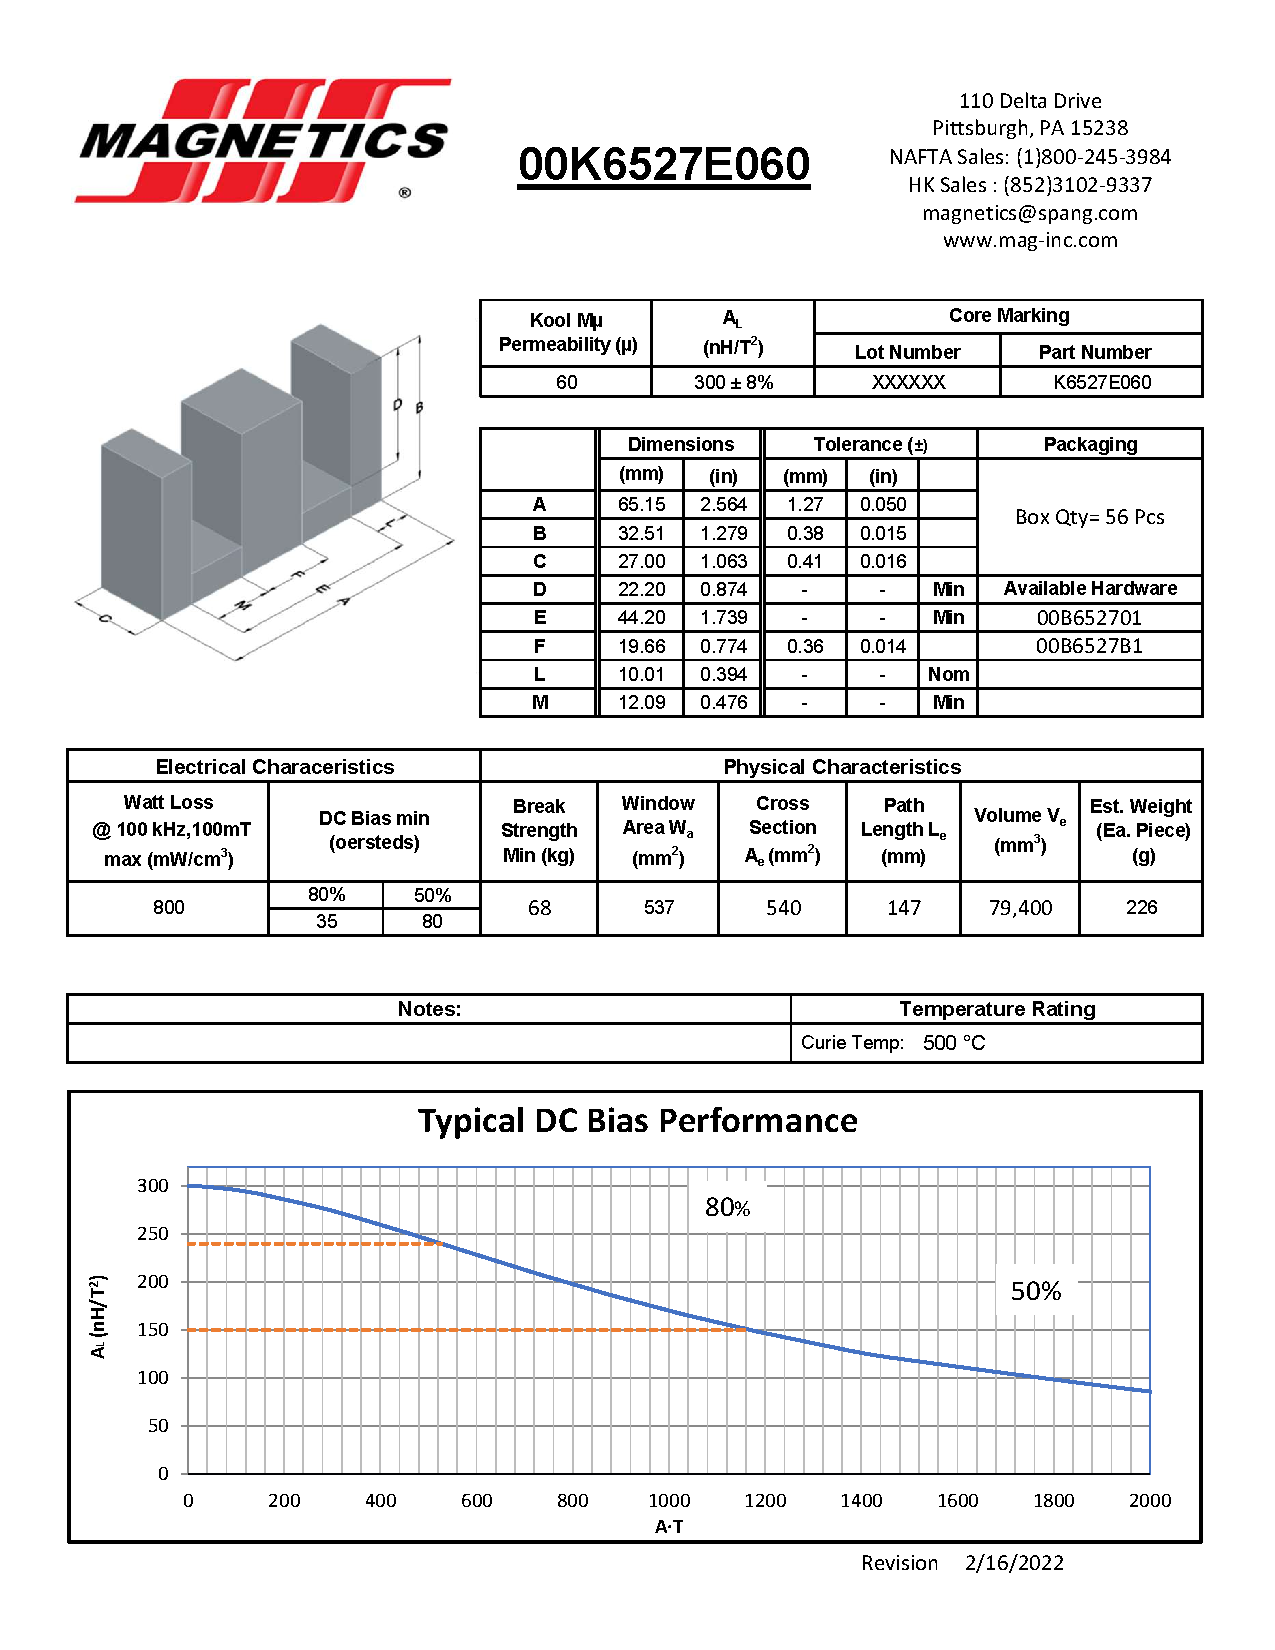
\includepdf[pages=-]{00K6527E060.pdf}
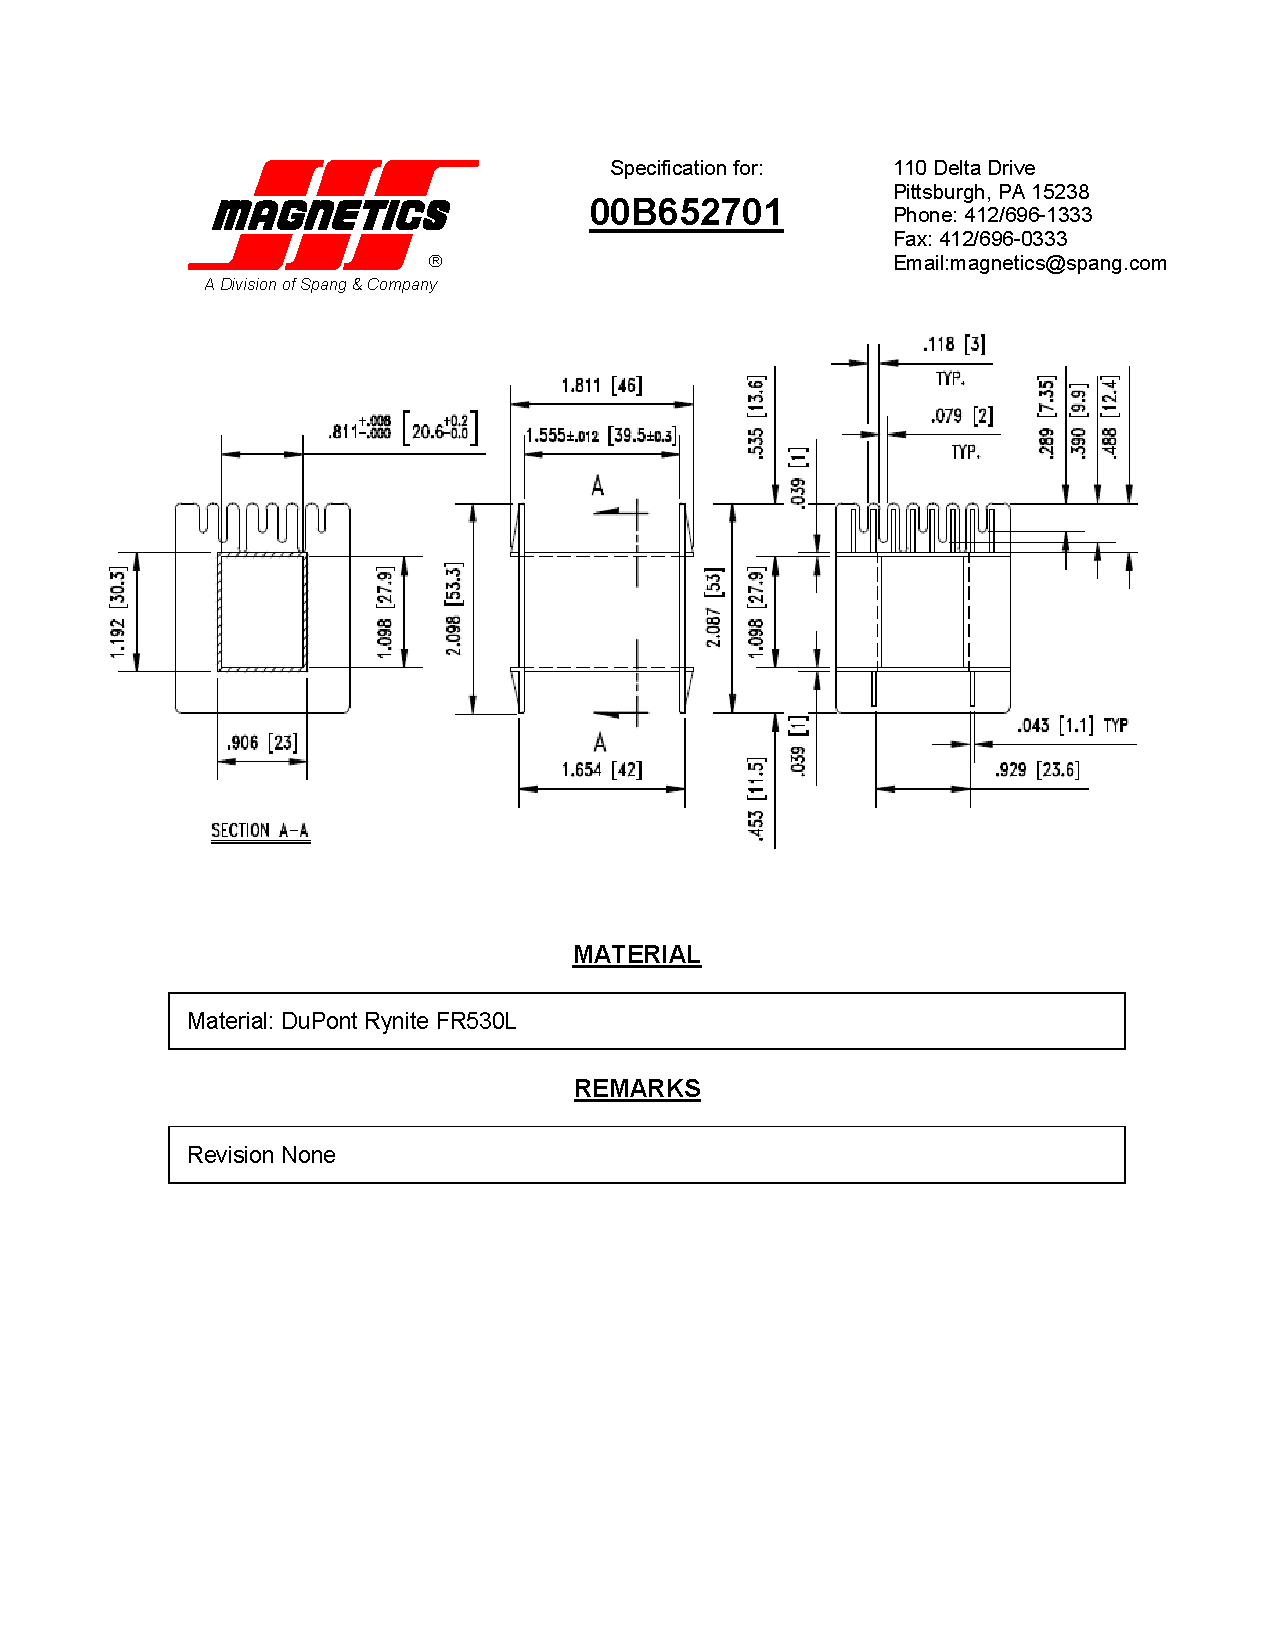
\includepdf[pages=-]{00B652701.pdf}

\section{RMS Value of a Non-symmetrical Triangle Wave with DC Bias}
\label{app:rmsderivation}
\subsection{Non-Symmetrical Triangle Wave with DC Bias}

This triangle wave is defined by
\[
I(t) = \begin{cases}
I_{\min} + \dfrac{I_{\max}-I_{\min}}{t_{\text{on}}}\,t, & 0\le t < t_{\text{on}}, \\[1mm]
I_{\max} - \dfrac{I_{\max}-I_{\min}}{t_{\text{off}}}\,(t-t_{\text{on}}), & t_{\text{on}}\le t < T,
\end{cases}
\]
where
\[
I_{\min} = I_{\text{bias}}\Bigl(1-\frac{\text{RF}}{2}\Bigr),\quad
I_{\max} = I_{\text{bias}}\Bigl(1+\frac{\text{RF}}{2}\Bigr),\quad
T = t_{\text{on}}+t_{\text{off}}.
\]
For example, if \(I_{\text{bias}}=50\,\text{A}\) and \(\text{RF}=0.4\), then
\[
I_{\min}=40\,\text{A}\quad \text{and}\quad I_{\max}=60\,\text{A}.
\]

Below is the plot of the triangle wave over three periods. In the code we set
\[
t_{\text{on}}=0.36,\quad t_{\text{off}}=0.64,\quad \text{so that} \quad T=1.0.
\]

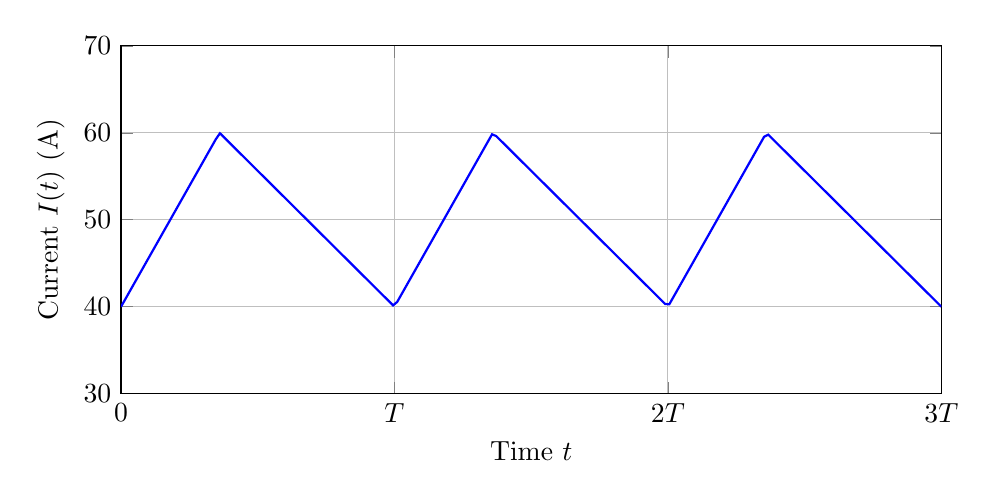
\begin{tikzpicture}
  % Define parameters
  \pgfmathsetmacro{\Ibias}{50}          % DC bias in A
  \pgfmathsetmacro{\RF}{0.4}             % Ripple factor (fraction)
  \pgfmathsetmacro{\Imin}{\Ibias - (\RF*\Ibias)/2} % Minimum current
  \pgfmathsetmacro{\Imax}{\Ibias + (\RF*\Ibias)/2} % Maximum current
  \pgfmathsetmacro{\ton}{0.36}            % On time (rising edge duration)
  \pgfmathsetmacro{\toff}{0.64}           % Off time (falling edge duration)
  \pgfmathsetmacro{\T}{\ton+\toff}       % Total period

  \begin{axis}[
      xlabel={Time \(t\)},
      ylabel={Current \(I(t)\) (A)},
      grid=both,
      width=12cm,
      height=6cm,
      xmin=0, xmax=3*\T,
      ymin=30, ymax=70,
      xtick={0,\T,2*\T,3*\T},
      xticklabels={\(0\),\(T\),\(2T\),\(3T\)},
      domain=0:3*\T,
      samples=200,
  ]
    % Plot the repeating triangle wave using modulo arithmetic.
    \addplot[blue, thick] 
      ({x}, { (mod(x,\T) < \ton) ? 
        (\Imin + (\Imax-\Imin)/\ton * mod(x,\T)) : 
        (\Imax - (\Imax-\Imin)/\toff * (mod(x,\T)-\ton)) });
  \end{axis}
\end{tikzpicture}

\subsection{RMS of Non-symmetrical Triangle Wave Derivation}
We are given a non-symmetrical triangle wave with zero mean defined by
\[
I(t) =
\begin{cases}
I_{\min} + \dfrac{I_{\max}-I_{\min}}{t_{\text{on}}}\,t, & 0\le t < t_{\text{on}}, \\[1mm]
I_{\max} - \dfrac{I_{\max}-I_{\min}}{t_{\text{off}}}\,(t-t_{\text{on}}), & t_{\text{on}}\le t < T,
\end{cases}
\]
with
\[
I_{\min} = -I_{\text{amplitude}}, \quad I_{\max} = I_{\text{amplitude}}, \quad t_{\text{on}} + t_{\text{off}} = T.
\]
The RMS value is defined as
\[
I_{\text{RMS}} = \sqrt{\frac{1}{T}\int_0^T [I(t)]^2\,dt}.
\]

\subsection{Rising Segment ($0\le t < t_{\text{on}}$)}

For the rising segment, substituting the given values yields
\[
I(t) = -I_{\text{amplitude}} + \frac{2I_{\text{amplitude}}}{t_{\text{on}}}\,t = I_{\text{amplitude}}\left(-1 + \frac{2t}{t_{\text{on}}}\right).
\]
Thus,
\[
[I(t)]^2 = I_{\text{amplitude}}^2 \left(-1 + \frac{2t}{t_{\text{on}}}\right)^2
= I_{\text{amplitude}}^2 \left(1 - \frac{4t}{t_{\text{on}}} + \frac{4t^2}{t_{\text{on}}^2}\right).
\]
Integrate over \(t\) from 0 to \(t_{\text{on}}\):
\begin{align*}
\int_0^{t_{\text{on}}} [I(t)]^2\, dt 
&= I_{\text{amplitude}}^2 \int_0^{t_{\text{on}}} \left(1 - \frac{4t}{t_{\text{on}}} + \frac{4t^2}{t_{\text{on}}^2}\right) dt \\
&= I_{\text{amplitude}}^2 \left[ \int_0^{t_{\text{on}}} dt - \frac{4}{t_{\text{on}}}\int_0^{t_{\text{on}}} t\,dt + \frac{4}{t_{\text{on}}^2}\int_0^{t_{\text{on}}} t^2\,dt \right] \\
&= I_{\text{amplitude}}^2 \left[ t_{\text{on}} - \frac{4}{t_{\text{on}}}\cdot\frac{t_{\text{on}}^2}{2} + \frac{4}{t_{\text{on}}^2}\cdot\frac{t_{\text{on}}^3}{3} \right] \\
&= I_{\text{amplitude}}^2 \left[ t_{\text{on}} - 2t_{\text{on}} + \frac{4t_{\text{on}}}{3} \right] \\
&= I_{\text{amplitude}}^2\,t_{\text{on}} \left(1 - 2 + \frac{4}{3}\right) \\
&= \frac{I_{\text{amplitude}}^2\,t_{\text{on}}}{3}.
\end{align*}

\subsection{Falling Segment ($t_{\text{on}}\le t < T$)}

For the falling segment,
\[
I(t) = I_{\text{amplitude}} - \frac{2I_{\text{amplitude}}}{t_{\text{off}}}(t-t_{\text{on}}) = I_{\text{amplitude}}\left[1 - \frac{2}{t_{\text{off}}}(t-t_{\text{on}})\right].
\]
Its square is
\[
[I(t)]^2 = I_{\text{amplitude}}^2\left[1 - \frac{2}{t_{\text{off}}}(t-t_{\text{on}})\right]^2.
\]
Introduce the substitution
\[
u = t-t_{\text{on}}, \quad du = dt, \quad u \in [0, t_{\text{off}}].
\]
Then,
\[
[I(t)]^2 = I_{\text{amplitude}}^2 \left(1 - \frac{2u}{t_{\text{off}}}\right)^2
= I_{\text{amplitude}}^2 \left(1 - \frac{4u}{t_{\text{off}}} + \frac{4u^2}{t_{\text{off}}^2}\right),
\]
and the integral becomes
\begin{align*}
\int_{t_{\text{on}}}^{T} [I(t)]^2\, dt 
&= I_{\text{amplitude}}^2 \int_0^{t_{\text{off}}} \left(1 - \frac{4u}{t_{\text{off}}} + \frac{4u^2}{t_{\text{off}}^2}\right) du \\
&= I_{\text{amplitude}}^2 \left[ \int_0^{t_{\text{off}}} du - \frac{4}{t_{\text{off}}}\int_0^{t_{\text{off}}} u\,du + \frac{4}{t_{\text{off}}^2}\int_0^{t_{\text{off}}} u^2\,du \right] \\
&= I_{\text{amplitude}}^2 \left[ t_{\text{off}} - \frac{4}{t_{\text{off}}}\cdot\frac{t_{\text{off}}^2}{2} + \frac{4}{t_{\text{off}}^2}\cdot\frac{t_{\text{off}}^3}{3} \right] \\
&= I_{\text{amplitude}}^2 \left[ t_{\text{off}} - 2t_{\text{off}} + \frac{4t_{\text{off}}}{3} \right] \\
&= I_{\text{amplitude}}^2\,t_{\text{off}} \left(1 - 2 + \frac{4}{3}\right) \\
&= \frac{I_{\text{amplitude}}^2\,t_{\text{off}}}{3}.
\end{align*}

\subsection{Total RMS Value}

The total integral over one period is
\[
\int_0^T [I(t)]^2\, dt = \frac{I_{\text{amplitude}}^2\,t_{\text{on}}}{3} + \frac{I_{\text{amplitude}}^2\,t_{\text{off}}}{3}
= \frac{I_{\text{amplitude}}^2}{3}\,(t_{\text{on}}+t_{\text{off}}).
\]
Since \(t_{\text{on}}+t_{\text{off}} = T\), it follows that
\[
\int_0^T [I(t)]^2\, dt = \frac{I_{\text{amplitude}}^2\,T}{3}.
\]
Thus, the RMS value is
\[
I_{\text{RMS}} = \sqrt{\frac{1}{T}\int_0^T [I(t)]^2\, dt}
= \sqrt{\frac{I_{\text{amplitude}}^2}{3}}
= \frac{I_{\text{amplitude}}}{\sqrt{3}}.
\]

\[
\boxed{ I_{\text{RMS}} = \frac{I_{\text{amplitude}}}{\sqrt{3}}. }
\]

Note that even though the waveform is non-symmetrical in time (i.e., \(t_{\text{on}} \neq t_{\text{off}}\)), the RMS value depends only on the amplitude when the mean is zero.

\subsection{RMS of Two Orthogonal Signals}

The DC offset and the triangle wave are orthogonal signals because the multiplication of the two functions integrates to zero over each period. This is because the triangle wave has a zero mean and the DC offset is a constant value. \\

Therefore,
\[
V_{\text{RMS, total}} = \sqrt{V_{\text{DC}}^2 + V_{\text{RMS, triangle}}^2}
\]

The RMS of a non-symmetrical triangle wave with DC offset is independent of D and is equal to:

\[
\boxed{I_{\text{RMS, total}} = \sqrt{I_{\text{DC}}^2 + \frac{I_\text{Amp}^2}{3}}}
\]

\printbibliography
\end{document}